\documentclass[twoside]{book}

% Packages required by doxygen
\usepackage{fixltx2e}
\usepackage{calc}
\usepackage{doxygen}
\usepackage[export]{adjustbox} % also loads graphicx
\usepackage{graphicx}
\usepackage[utf8]{inputenc}
\usepackage{makeidx}
\usepackage{multicol}
\usepackage{multirow}
\PassOptionsToPackage{warn}{textcomp}
\usepackage{textcomp}
\usepackage[nointegrals]{wasysym}
\usepackage[table]{xcolor}

% NLS support packages
\usepackage[french]{babel}

% Font selection
\usepackage[T1]{fontenc}
\usepackage[scaled=.90]{helvet}
\usepackage{courier}
\usepackage{amssymb}
\usepackage{sectsty}
\renewcommand{\familydefault}{\sfdefault}
\allsectionsfont{%
  \fontseries{bc}\selectfont%
  \color{darkgray}%
}
\renewcommand{\DoxyLabelFont}{%
  \fontseries{bc}\selectfont%
  \color{darkgray}%
}
\newcommand{\+}{\discretionary{\mbox{\scriptsize$\hookleftarrow$}}{}{}}

% Page & text layout
\usepackage{geometry}
\geometry{%
  a4paper,%
  top=2.5cm,%
  bottom=2.5cm,%
  left=2.5cm,%
  right=2.5cm%
}
\tolerance=750
\hfuzz=15pt
\hbadness=750
\setlength{\emergencystretch}{15pt}
\setlength{\parindent}{0cm}
\setlength{\parskip}{3ex plus 2ex minus 2ex}
\makeatletter
\renewcommand{\paragraph}{%
  \@startsection{paragraph}{4}{0ex}{-1.0ex}{1.0ex}{%
    \normalfont\normalsize\bfseries\SS@parafont%
  }%
}
\renewcommand{\subparagraph}{%
  \@startsection{subparagraph}{5}{0ex}{-1.0ex}{1.0ex}{%
    \normalfont\normalsize\bfseries\SS@subparafont%
  }%
}
\makeatother

% Headers & footers
\usepackage{fancyhdr}
\pagestyle{fancyplain}
\fancyhead[LE]{\fancyplain{}{\bfseries\thepage}}
\fancyhead[CE]{\fancyplain{}{}}
\fancyhead[RE]{\fancyplain{}{\bfseries\leftmark}}
\fancyhead[LO]{\fancyplain{}{\bfseries\rightmark}}
\fancyhead[CO]{\fancyplain{}{}}
\fancyhead[RO]{\fancyplain{}{\bfseries\thepage}}
\fancyfoot[LE]{\fancyplain{}{}}
\fancyfoot[CE]{\fancyplain{}{}}
\fancyfoot[RE]{\fancyplain{}{\bfseries\scriptsize Généré par Doxygen }}
\fancyfoot[LO]{\fancyplain{}{\bfseries\scriptsize Généré par Doxygen }}
\fancyfoot[CO]{\fancyplain{}{}}
\fancyfoot[RO]{\fancyplain{}{}}
\renewcommand{\footrulewidth}{0.4pt}
\renewcommand{\chaptermark}[1]{%
  \markboth{#1}{}%
}
\renewcommand{\sectionmark}[1]{%
  \markright{\thesection\ #1}%
}

% Indices & bibliography
\usepackage{natbib}
\usepackage[titles]{tocloft}
\setcounter{tocdepth}{3}
\setcounter{secnumdepth}{5}
\makeindex

% Hyperlinks (required, but should be loaded last)
\usepackage{ifpdf}
\ifpdf
  \usepackage[pdftex,pagebackref=true]{hyperref}
\else
  \usepackage[ps2pdf,pagebackref=true]{hyperref}
\fi
\hypersetup{%
  colorlinks=true,%
  linkcolor=blue,%
  citecolor=blue,%
  unicode%
}

% Custom commands
\newcommand{\clearemptydoublepage}{%
  \newpage{\pagestyle{empty}\cleardoublepage}%
}

\usepackage{caption}
\captionsetup{labelsep=space,justification=centering,font={bf},singlelinecheck=off,skip=4pt,position=top}

%===== C O N T E N T S =====

\begin{document}

% Titlepage & ToC
\hypersetup{pageanchor=false,
             bookmarksnumbered=true,
             pdfencoding=unicode
            }
\pagenumbering{roman}
\begin{titlepage}
\vspace*{7cm}
\begin{center}%
{\Large Projet\+C\+I\+R2\+:monitoring \\[1ex]\large 1.\+0 }\\
\vspace*{1cm}
{\large Généré par Doxygen 1.8.11}\\
\end{center}
\end{titlepage}
\clearemptydoublepage
\tableofcontents
\clearemptydoublepage
\pagenumbering{arabic}
\hypersetup{pageanchor=true}

%--- Begin generated contents ---
\chapter{Liste des bogues}
\label{bug}
\hypertarget{bug}{}

\begin{DoxyRefList}
\item[\label{bug__bug000001}%
\hypertarget{bug__bug000001}{}%
Classe \hyperlink{classDataBase}{Data\+Base} ]L\textquotesingle{}envoi de mails aurait pû faire l\textquotesingle{}objet d\textquotesingle{}une méthode de cette classe mais la bibliotheque choisie n\textquotesingle{}a pas permis cela. 
\end{DoxyRefList}
\chapter{Index hiérarchique}
\section{Hiérarchie des classes}
Cette liste d\textquotesingle{}héritage est classée approximativement par ordre alphabétique \+:\begin{DoxyCompactList}
\item Connection\begin{DoxyCompactList}
\item \contentsline{section}{sql\+:\+:mysql\+:\+:My\+S\+Q\+L\+\_\+\+Connection}{\pageref{classsql_1_1mysql_1_1MySQL__Connection}}{}
\end{DoxyCompactList}
\item \contentsline{section}{Data\+Base}{\pageref{classDataBase}}{}
\item Q\+Object\begin{DoxyCompactList}
\item \contentsline{section}{Echo\+Client}{\pageref{classEchoClient}}{}
\end{DoxyCompactList}
\item \contentsline{section}{qt\+\_\+meta\+\_\+stringdata\+\_\+\+Echo\+Client\+\_\+t}{\pageref{structqt__meta__stringdata__EchoClient__t}}{}
\item Savepoint\begin{DoxyCompactList}
\item \contentsline{section}{sql\+:\+:mysql\+:\+:My\+S\+Q\+L\+\_\+\+Savepoint}{\pageref{classsql_1_1mysql_1_1MySQL__Savepoint}}{}
\end{DoxyCompactList}
\end{DoxyCompactList}

\chapter{Index des classes}
\section{Liste des classes}
Liste des classes, structures, unions et interfaces avec une brève description \+:\begin{DoxyCompactList}
\item\contentsline{section}{\hyperlink{classDataBase}{Data\+Base} \\*La classe {\bfseries \hyperlink{classDataBase}{Data\+Base}} sert à intéragir avec la base de données }{\pageref{classDataBase}}{}
\item\contentsline{section}{\hyperlink{classEchoClient}{Echo\+Client} \\*La classe {\bfseries \hyperlink{classEchoClient}{Echo\+Client}} est l\textquotesingle{}ensemble des fonctionnalités permettant de récupérer une trame et de la traiter }{\pageref{classEchoClient}}{}
\item\contentsline{section}{\hyperlink{classsql_1_1mysql_1_1MySQL__Connection}{sql\+::mysql\+::\+My\+S\+Q\+L\+\_\+\+Connection} }{\pageref{classsql_1_1mysql_1_1MySQL__Connection}}{}
\item\contentsline{section}{\hyperlink{classsql_1_1mysql_1_1MySQL__Savepoint}{sql\+::mysql\+::\+My\+S\+Q\+L\+\_\+\+Savepoint} }{\pageref{classsql_1_1mysql_1_1MySQL__Savepoint}}{}
\item\contentsline{section}{\hyperlink{structqt__meta__stringdata__EchoClient__t}{qt\+\_\+meta\+\_\+stringdata\+\_\+\+Echo\+Client\+\_\+t} }{\pageref{structqt__meta__stringdata__EchoClient__t}}{}
\end{DoxyCompactList}

\chapter{Index des fichiers}
\section{Liste des fichiers}
Liste de tous les fichiers documentés avec une brève description \+:\begin{DoxyCompactList}
\item\contentsline{section}{\hyperlink{database_8cpp}{database.\+cpp} }{\pageref{database_8cpp}}{}
\item\contentsline{section}{{\bfseries database.\+h} }{\pageref{database_8h}}{}
\item\contentsline{section}{\hyperlink{echoclient_8cpp}{echoclient.\+cpp} }{\pageref{echoclient_8cpp}}{}
\item\contentsline{section}{\hyperlink{echoclient_8h}{echoclient.\+h} \\*Le fichier d\textquotesingle{}en-\/tête de la classe {\bfseries \hyperlink{classDataBase}{Data\+Base}} }{\pageref{echoclient_8h}}{}
\item\contentsline{section}{\hyperlink{main_8cpp}{main.\+cpp} }{\pageref{main_8cpp}}{}
\item\contentsline{section}{{\bfseries mysql\+\_\+connection.\+h} }{\pageref{mysql__connection_8h}}{}
\end{DoxyCompactList}

\chapter{Documentation des classes}
\hypertarget{classDataBase}{}\section{Référence de la classe Data\+Base}
\label{classDataBase}\index{Data\+Base@{Data\+Base}}


La classe {\bfseries \hyperlink{classDataBase}{Data\+Base}} sert à intéragir avec la base de données.  




{\ttfamily \#include $<$database.\+h$>$}

\subsection*{Fonctions membres publiques}
\begin{DoxyCompactItemize}
\item 
\hyperlink{classDataBase_a58bcabfc07dc77eb0fc35d27523f3e9f}{Data\+Base} (string path, string login, string pass, Q\+String time, int temperature, int humidite, Q\+String user, Q\+String four, double C\+O2, int chute, Q\+String tv, Q\+String pas, string id\+\_\+room)
\begin{DoxyCompactList}\small\item\em Le constructeur de la classe {\bfseries \hyperlink{classDataBase}{Data\+Base}}. \end{DoxyCompactList}\item 
void \hyperlink{classDataBase_a65ad879d829e20db4a78719e62c8356e}{Comparaison} (string path, string login, string pass, Q\+String time, int temperature, int humidite, Q\+String user, Q\+String four, double C\+O2, int chute, Q\+String tv, string id\+\_\+room)
\item 
void \hyperlink{classDataBase_aa1c151b2f7d0adb2a2a7a692db65e3f4}{create\+Alert} (string path, string login, string pass, Q\+String user, Q\+String time, int type, int sens\+Depassement, int value, string id\+\_\+room)
\begin{DoxyCompactList}\small\item\em Cette méthode peut être appelée par {\bfseries \hyperlink{classDataBase_a65ad879d829e20db4a78719e62c8356e}{Comparaison()}} dans la cas de dépassement d\textquotesingle{}un seuil. \end{DoxyCompactList}\end{DoxyCompactItemize}


\subsection{Description détaillée}
La classe {\bfseries \hyperlink{classDataBase}{Data\+Base}} sert à intéragir avec la base de données. 

Ses fonctionnalités consistent à envoyer les valeurs reçues et traitées dans {\bfseries \hyperlink{classEchoClient}{Echo\+Client}} dans la base de données, mais aussi à récupérer les données de seuils pour les comparer avec les valeurs de la trame actuelle. Si un dépassement est constaté, une alerte sera créée et envoyée dans l\textquotesingle{}entité correspondante de la base de données. \begin{DoxyRefDesc}{Bogue}
\item[\hyperlink{bug__bug000001}{Bogue}]L\textquotesingle{}envoi de mails aurait pû faire l\textquotesingle{}objet d\textquotesingle{}une méthode de cette classe mais la bibliotheque choisie n\textquotesingle{}a pas permis cela. \end{DoxyRefDesc}


\subsection{Documentation des constructeurs et destructeur}
\index{Data\+Base@{Data\+Base}!Data\+Base@{Data\+Base}}
\index{Data\+Base@{Data\+Base}!Data\+Base@{Data\+Base}}
\subsubsection[{\texorpdfstring{Data\+Base(string path, string login, string pass, Q\+String time, int temperature, int humidite, Q\+String user, Q\+String four, double C\+O2, int chute, Q\+String tv, Q\+String pas, string id\+\_\+room)}{DataBase(string path, string login, string pass, QString time, int temperature, int humidite, QString user, QString four, double CO2, int chute, QString tv, QString pas, string id_room)}}]{\setlength{\rightskip}{0pt plus 5cm}Data\+Base\+::\+Data\+Base (
\begin{DoxyParamCaption}
\item[{string}]{path, }
\item[{string}]{login, }
\item[{string}]{pass, }
\item[{Q\+String}]{time, }
\item[{int}]{temperature, }
\item[{int}]{humidite, }
\item[{Q\+String}]{user, }
\item[{Q\+String}]{four, }
\item[{double}]{C\+O2, }
\item[{int}]{chute, }
\item[{Q\+String}]{tv, }
\item[{Q\+String}]{pas, }
\item[{string}]{id\+\_\+room}
\end{DoxyParamCaption}
)}\hypertarget{classDataBase_a58bcabfc07dc77eb0fc35d27523f3e9f}{}\label{classDataBase_a58bcabfc07dc77eb0fc35d27523f3e9f}


Le constructeur de la classe {\bfseries \hyperlink{classDataBase}{Data\+Base}}. 

En fonction des données qui lui sont transmises, il remplira l\textquotesingle{}entité {\bfseries V\+A\+L\+UE} de la base de données. Si les quatres valeurs numériques de la trame des chambres sont à 0, il va gérer les données utilisateur (nombre de pas...) Dans le cas contraire, ce sont les données des chambres qui lui sont envoyées. Dans les deux cas, une requête I\+N\+S\+E\+RT I\+N\+TO V\+A\+L\+UE(...) V\+A\+L\+U\+ES(...) sera envoyée à la base de données. 
\begin{DoxyParams}{Paramètres}
{\em path} & L\textquotesingle{}adresse de la base de données. \\
\hline
{\em login} & L\textquotesingle{}identifiant pour se connecter à al base de données. \\
\hline
{\em pass} & Le mot de passe pour se connecter à la base de données. \\
\hline
{\em time} & La date et l\textquotesingle{}heure \\
\hline
{\em temperature} & La valeur de la temperature. \\
\hline
{\em humidite} & La valeur de l\textquotesingle{}humidité en \% \\
\hline
{\em user} & L\textquotesingle{}adresse mail de l\textquotesingle{}utilisateur de la pièce. \\
\hline
{\em four} & La valeur associée à la mise en marche du four. \\
\hline
{\em C\+O2} & La valeur du taux de C\+O2 en ppm. \\
\hline
{\em chute} & La valeur associée à l\textquotesingle{}éventuelle chute de l\textquotesingle{}utilisateur \\
\hline
{\em tv} & La valeur associée à l\textquotesingle{}allumage de la télévision \\
\hline
{\em pas} & Le nombre de pas effectués par l\textquotesingle{}utilisateur pendant la dernière heure. \\
\hline
{\em id\+\_\+room} & Le numero de la pièce. \\
\hline
\end{DoxyParams}


\subsection{Documentation des fonctions membres}
\index{Data\+Base@{Data\+Base}!Comparaison@{Comparaison}}
\index{Comparaison@{Comparaison}!Data\+Base@{Data\+Base}}
\subsubsection[{\texorpdfstring{Comparaison(string path, string login, string pass, Q\+String time, int temperature, int humidite, Q\+String user, Q\+String four, double C\+O2, int chute, Q\+String tv, string id\+\_\+room)}{Comparaison(string path, string login, string pass, QString time, int temperature, int humidite, QString user, QString four, double CO2, int chute, QString tv, string id_room)}}]{\setlength{\rightskip}{0pt plus 5cm}Data\+Base\+::\+Comparaison (
\begin{DoxyParamCaption}
\item[{string}]{path, }
\item[{string}]{login, }
\item[{string}]{pass, }
\item[{Q\+String}]{time, }
\item[{int}]{temperature, }
\item[{int}]{humidite, }
\item[{Q\+String}]{user, }
\item[{Q\+String}]{four, }
\item[{double}]{C\+O2, }
\item[{int}]{chute, }
\item[{Q\+String}]{tv, }
\item[{string}]{id\+\_\+room}
\end{DoxyParamCaption}
)}\hypertarget{classDataBase_a65ad879d829e20db4a78719e62c8356e}{}\label{classDataBase_a65ad879d829e20db4a78719e62c8356e}
Cette méthode consiste à envoyer une requête S\+E\+L\+E\+CT ... F\+R\+OM ... W\+H\+E\+RE pour récupérer les seuils propres à chaque capteur. Les valeurs passées en paramètres sont ensuite comparées avec leurs seuils respectifs, dès qu\textquotesingle{}un dépassement est constaté, un appel est lancé à la méthode \hyperlink{classDataBase_aa1c151b2f7d0adb2a2a7a692db65e3f4}{create\+Alert()}. 
\begin{DoxyParams}{Paramètres}
{\em path} & L\textquotesingle{}adresse de la base de données. \\
\hline
{\em login} & L\textquotesingle{}identifiant pour se connecter à al base de données. \\
\hline
{\em pass} & Le mot de passe pour se connecter à la base de données. \\
\hline
{\em time} & La date et l\textquotesingle{}heure. \\
\hline
{\em temperature} & La valeur de la temperature. \\
\hline
{\em humidite} & La valeur de l\textquotesingle{}humidité en \%. \\
\hline
{\em user} & L\textquotesingle{}adresse mail de l\textquotesingle{}utilisateur de la pièce. \\
\hline
{\em four} & La valeur associée à la mise en marche du four. \\
\hline
{\em C\+O2} & La valeur du taux de C\+O2 en ppm. \\
\hline
{\em chute} & La valeur associée à l\textquotesingle{}éventuelle chute de l\textquotesingle{}utilisateur. \\
\hline
{\em tv} & La valeur associée à l\textquotesingle{}allumage de la télévision. \\
\hline
\end{DoxyParams}
\index{Data\+Base@{Data\+Base}!create\+Alert@{create\+Alert}}
\index{create\+Alert@{create\+Alert}!Data\+Base@{Data\+Base}}
\subsubsection[{\texorpdfstring{create\+Alert(string path, string login, string pass, Q\+String user, Q\+String time, int type, int sens\+Depassement, int value, string id\+\_\+room)}{createAlert(string path, string login, string pass, QString user, QString time, int type, int sensDepassement, int value, string id_room)}}]{\setlength{\rightskip}{0pt plus 5cm}Data\+Base\+::create\+Alert (
\begin{DoxyParamCaption}
\item[{string}]{path, }
\item[{string}]{login, }
\item[{string}]{pass, }
\item[{Q\+String}]{user, }
\item[{Q\+String}]{time, }
\item[{int}]{type, }
\item[{int}]{sens\+Depassement, }
\item[{int}]{value, }
\item[{string}]{id\+\_\+room}
\end{DoxyParamCaption}
)}\hypertarget{classDataBase_aa1c151b2f7d0adb2a2a7a692db65e3f4}{}\label{classDataBase_aa1c151b2f7d0adb2a2a7a692db65e3f4}


Cette méthode peut être appelée par {\bfseries \hyperlink{classDataBase_a65ad879d829e20db4a78719e62c8356e}{Comparaison()}} dans la cas de dépassement d\textquotesingle{}un seuil. 

En fonction du type d\textquotesingle{}alerte (ou plutôt du capteur qui la déclenche), la description de l\textquotesingle{}alerte changera. une requête I\+N\+S\+E\+RT I\+N\+TO est ensuite envoyée pour ajouter les données liées à l\textquotesingle{}alerte dans l\textquotesingle{}entité A\+L\+E\+R\+TE de la base de données. 
\begin{DoxyParams}{Paramètres}
{\em path} & L\textquotesingle{}adresse de la base de données. \\
\hline
{\em login} & L\textquotesingle{}identifiant pour se connecter à al base de données. \\
\hline
{\em pass} & Le mot de passe pour se connecter à la base de données. \\
\hline
{\em time} & La date et l\textquotesingle{}heure. \\
\hline
{\em type} & Le type de capteur concerné. \\
\hline
{\em sens\+Depassement} & Une variable qui permet de savoir si c\textquotesingle{}est le seuil haut ou bas qui a été dépassé. \\
\hline
{\em value} & La valeur envoyée par le capteur. \\
\hline
{\em id\+\_\+room} & Le numero de la pièce. \\
\hline
\end{DoxyParams}


La documentation de cette classe a été générée à partir des fichiers suivants \+:\begin{DoxyCompactItemize}
\item 
database.\+h\item 
\hyperlink{database_8cpp}{database.\+cpp}\end{DoxyCompactItemize}

\hypertarget{classEchoClient}{}\section{Référence de la classe Echo\+Client}
\label{classEchoClient}\index{Echo\+Client@{Echo\+Client}}


La classe {\bfseries \hyperlink{classEchoClient}{Echo\+Client}} est l\textquotesingle{}ensemble des fonctionnalités permettant de récupérer une trame et de la traiter.  




{\ttfamily \#include $<$echoclient.\+h$>$}



Graphe d\textquotesingle{}héritage de Echo\+Client\+:\nopagebreak
\begin{figure}[H]
\begin{center}
\leavevmode
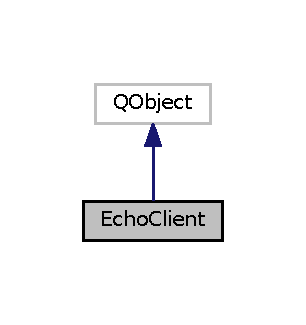
\includegraphics[width=147pt]{classEchoClient__inherit__graph}
\end{center}
\end{figure}


Graphe de collaboration de Echo\+Client\+:\nopagebreak
\begin{figure}[H]
\begin{center}
\leavevmode
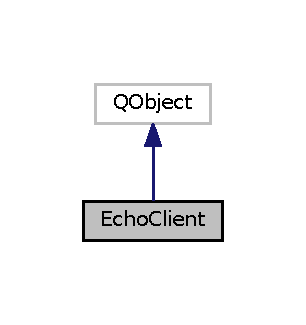
\includegraphics[width=147pt]{classEchoClient__coll__graph}
\end{center}
\end{figure}
\subsection*{Signaux}
\begin{DoxyCompactItemize}
\item 
void {\bfseries closed} ()\hypertarget{classEchoClient_a0834d7f65bf0ed5411573ef34bf638e7}{}\label{classEchoClient_a0834d7f65bf0ed5411573ef34bf638e7}

\end{DoxyCompactItemize}
\subsection*{Fonctions membres publiques}
\begin{DoxyCompactItemize}
\item 
\hyperlink{classEchoClient_a77a327e3a287f5797820cd5265164593}{Echo\+Client} (const Q\+Url \&url, bool debug=false, Q\+Object $\ast$parent=Q\+\_\+\+N\+U\+L\+L\+P\+TR)
\begin{DoxyCompactList}\small\item\em Constructeur de la classe \hyperlink{classEchoClient}{Echo\+Client}. \end{DoxyCompactList}\item 
void \hyperlink{classEchoClient_ac834f3a4331b8a0674a3614cf4513b9a}{traitement\+Chambre} (Q\+String message)
\begin{DoxyCompactList}\small\item\em Fonction qui sépare les éléments de la trame de la pièce, les traite et les envoie à la base de données. \end{DoxyCompactList}\item 
void \hyperlink{classEchoClient_a79508ca23964331b9b189a5282245d2d}{traitement\+Utilisateur} (Q\+String message)
\begin{DoxyCompactList}\small\item\em Fonction qui sépare les éléments de la trame utilisateur, les traite et les envoie à la base de données. \end{DoxyCompactList}\item 
int \hyperlink{classEchoClient_acf8a95fc397766e5429fc2cf7bd1f54d}{decode\+M\+T\+H\+O2} (Q\+String mtho2)
\begin{DoxyCompactList}\small\item\em Fonction qui extrait la temperature de la chaine envoyée par le capteur M\+T\+H\+O2. \end{DoxyCompactList}\item 
int \hyperlink{classEchoClient_ab22fb89d56621f22e7547ed365f94bb5}{decode\+Humidity} (Q\+String qstr\+\_\+humidity)
\begin{DoxyCompactList}\small\item\em Fonction qui extrait le niveau d\textquotesingle{}humidité de la chaine envoyée par le capteur M\+T\+H\+O2. \end{DoxyCompactList}\item 
Q\+String \hyperlink{classEchoClient_a2463696ad18476d25d9e8eac47e65436}{decode\+Time} (double dtime)
\begin{DoxyCompactList}\small\item\em Fonction qui décode la timestamp entré et renvoie l\textquotesingle{}heure en format lisible. \end{DoxyCompactList}\item 
string \hyperlink{classEchoClient_a2f6bc3131e02cbbcf3d422b08ec88185}{ask\+Bdd\+Ip} ()
\begin{DoxyCompactList}\small\item\em Fonction setter qui demande à l\textquotesingle{}utilisateur l\textquotesingle{}adresse IP et le port de la base de données. \end{DoxyCompactList}\item 
string \hyperlink{classEchoClient_ad6b9cddeae9043d79bf482da303c4b21}{ask\+Bdd\+Login} ()
\begin{DoxyCompactList}\small\item\em Fonction setter qui demande à l\textquotesingle{}utilisateur son identifiant pour se connecter à la base de données. \end{DoxyCompactList}\item 
string \hyperlink{classEchoClient_a7c8ccafa27fff1427fedae3fa8327e6e}{ask\+Bdd\+Password} ()
\begin{DoxyCompactList}\small\item\em Fonction setter qui demande à l\textquotesingle{}utilisateur le mot de passe pour se connecter à la base de données. \end{DoxyCompactList}\item 
string \hyperlink{classEchoClient_a80d1d6acbdc39d74740bf0e66c6e4c27}{ask\+Id\+Room} ()
\begin{DoxyCompactList}\small\item\em Fonction setter qui demande à l\textquotesingle{}utilisateur la pièce à laquelle est associée l\textquotesingle{}addresse IP rentrée plus tôt. \end{DoxyCompactList}\item 
string \hyperlink{classEchoClient_a3f7731443eebfdb9dc3484aa9f44d0db}{get\+Bdd\+Ip} ()
\begin{DoxyCompactList}\small\item\em Fonction getter retournant l\textquotesingle{}addresse de la base de données sous forme de chaine de caractères. \end{DoxyCompactList}\item 
string \hyperlink{classEchoClient_a4e8b1f06f6149d913b87786d0b926c2b}{get\+Bdd\+Login} ()
\begin{DoxyCompactList}\small\item\em Fonction getter retournant le login de la base de données sous forme de chaine de caractères. \end{DoxyCompactList}\item 
string \hyperlink{classEchoClient_afefb25861ae733ed0b74ace091843ab3}{get\+Bdd\+Password} ()
\begin{DoxyCompactList}\small\item\em Fonction getter retournant le mot de passe de la base de données sous forme de chaine de caractères. \end{DoxyCompactList}\item 
string \hyperlink{classEchoClient_a7c173d78a32ebadb5bd8320ebcef25b9}{get\+Id\+Room} ()
\begin{DoxyCompactList}\small\item\em Fonction getter retournant le numero de la pièce sous forme de chaine de caractères. \end{DoxyCompactList}\end{DoxyCompactItemize}


\subsection{Description détaillée}
La classe {\bfseries \hyperlink{classEchoClient}{Echo\+Client}} est l\textquotesingle{}ensemble des fonctionnalités permettant de récupérer une trame et de la traiter. 

\subsection{Documentation des constructeurs et destructeur}
\index{Echo\+Client@{Echo\+Client}!Echo\+Client@{Echo\+Client}}
\index{Echo\+Client@{Echo\+Client}!Echo\+Client@{Echo\+Client}}
\subsubsection[{\texorpdfstring{Echo\+Client(const Q\+Url \&url, bool debug=false, Q\+Object $\ast$parent=\+Q\+\_\+\+N\+U\+L\+L\+P\+T\+R)}{EchoClient(const QUrl &url, bool debug=false, QObject *parent=Q_NULLPTR)}}]{\setlength{\rightskip}{0pt plus 5cm}Echo\+Client\+::\+Echo\+Client (
\begin{DoxyParamCaption}
\item[{const Q\+Url \&}]{url, }
\item[{bool}]{debug = {\ttfamily false}, }
\item[{Q\+Object $\ast$}]{parent = {\ttfamily Q\+\_\+NULLPTR}}
\end{DoxyParamCaption}
)\hspace{0.3cm}{\ttfamily [explicit]}}\hypertarget{classEchoClient_a77a327e3a287f5797820cd5265164593}{}\label{classEchoClient_a77a327e3a287f5797820cd5265164593}


Constructeur de la classe \hyperlink{classEchoClient}{Echo\+Client}. 


\begin{DoxyParams}{Paramètres}
{\em \&url} & \\
\hline
{\em debug} & \\
\hline
{\em $\ast$parent} & \\
\hline
\end{DoxyParams}


\subsection{Documentation des fonctions membres}
\index{Echo\+Client@{Echo\+Client}!ask\+Bdd\+Ip@{ask\+Bdd\+Ip}}
\index{ask\+Bdd\+Ip@{ask\+Bdd\+Ip}!Echo\+Client@{Echo\+Client}}
\subsubsection[{\texorpdfstring{ask\+Bdd\+Ip()}{askBddIp()}}]{\setlength{\rightskip}{0pt plus 5cm}string Echo\+Client\+::ask\+Bdd\+Ip (
\begin{DoxyParamCaption}
{}
\end{DoxyParamCaption}
)}\hypertarget{classEchoClient_a2f6bc3131e02cbbcf3d422b08ec88185}{}\label{classEchoClient_a2f6bc3131e02cbbcf3d422b08ec88185}


Fonction setter qui demande à l\textquotesingle{}utilisateur l\textquotesingle{}adresse IP et le port de la base de données. 

\begin{DoxyReturn}{Renvoie}
Adresse de la base de données (std\+::string). 
\end{DoxyReturn}
\index{Echo\+Client@{Echo\+Client}!ask\+Bdd\+Login@{ask\+Bdd\+Login}}
\index{ask\+Bdd\+Login@{ask\+Bdd\+Login}!Echo\+Client@{Echo\+Client}}
\subsubsection[{\texorpdfstring{ask\+Bdd\+Login()}{askBddLogin()}}]{\setlength{\rightskip}{0pt plus 5cm}string Echo\+Client\+::ask\+Bdd\+Login (
\begin{DoxyParamCaption}
{}
\end{DoxyParamCaption}
)}\hypertarget{classEchoClient_ad6b9cddeae9043d79bf482da303c4b21}{}\label{classEchoClient_ad6b9cddeae9043d79bf482da303c4b21}


Fonction setter qui demande à l\textquotesingle{}utilisateur son identifiant pour se connecter à la base de données. 

\begin{DoxyReturn}{Renvoie}
L\textquotesingle{}identifiant permettant de se connecter à la base de données (std\+::string). 
\end{DoxyReturn}
\index{Echo\+Client@{Echo\+Client}!ask\+Bdd\+Password@{ask\+Bdd\+Password}}
\index{ask\+Bdd\+Password@{ask\+Bdd\+Password}!Echo\+Client@{Echo\+Client}}
\subsubsection[{\texorpdfstring{ask\+Bdd\+Password()}{askBddPassword()}}]{\setlength{\rightskip}{0pt plus 5cm}string Echo\+Client\+::ask\+Bdd\+Password (
\begin{DoxyParamCaption}
{}
\end{DoxyParamCaption}
)}\hypertarget{classEchoClient_a7c8ccafa27fff1427fedae3fa8327e6e}{}\label{classEchoClient_a7c8ccafa27fff1427fedae3fa8327e6e}


Fonction setter qui demande à l\textquotesingle{}utilisateur le mot de passe pour se connecter à la base de données. 

\begin{DoxyReturn}{Renvoie}
Le mot de passe permettant de se connecter à la base de données (std\+::string). 
\end{DoxyReturn}
\index{Echo\+Client@{Echo\+Client}!ask\+Id\+Room@{ask\+Id\+Room}}
\index{ask\+Id\+Room@{ask\+Id\+Room}!Echo\+Client@{Echo\+Client}}
\subsubsection[{\texorpdfstring{ask\+Id\+Room()}{askIdRoom()}}]{\setlength{\rightskip}{0pt plus 5cm}string Echo\+Client\+::ask\+Id\+Room (
\begin{DoxyParamCaption}
{}
\end{DoxyParamCaption}
)}\hypertarget{classEchoClient_a80d1d6acbdc39d74740bf0e66c6e4c27}{}\label{classEchoClient_a80d1d6acbdc39d74740bf0e66c6e4c27}


Fonction setter qui demande à l\textquotesingle{}utilisateur la pièce à laquelle est associée l\textquotesingle{}addresse IP rentrée plus tôt. 

\begin{DoxyReturn}{Renvoie}
Le numero de la pièce surveillée (std\+::string). 
\end{DoxyReturn}
\index{Echo\+Client@{Echo\+Client}!decode\+Humidity@{decode\+Humidity}}
\index{decode\+Humidity@{decode\+Humidity}!Echo\+Client@{Echo\+Client}}
\subsubsection[{\texorpdfstring{decode\+Humidity(\+Q\+String qstr\+\_\+humidity)}{decodeHumidity(QString qstr_humidity)}}]{\setlength{\rightskip}{0pt plus 5cm}int Echo\+Client\+::decode\+Humidity (
\begin{DoxyParamCaption}
\item[{Q\+String}]{qstr\+\_\+humidity}
\end{DoxyParamCaption}
)}\hypertarget{classEchoClient_ab22fb89d56621f22e7547ed365f94bb5}{}\label{classEchoClient_ab22fb89d56621f22e7547ed365f94bb5}


Fonction qui extrait le niveau d\textquotesingle{}humidité de la chaine envoyée par le capteur M\+T\+H\+O2. 


\begin{DoxyParams}{Paramètres}
{\em qstr\+\_\+humidity} & Chaine binaire envoyée par le capteur M\+T\+H\+O2. \\
\hline
\end{DoxyParams}
\begin{DoxyReturn}{Renvoie}
Le taux d\textquotesingle{}humidité de la pièce (int). 
\end{DoxyReturn}
\index{Echo\+Client@{Echo\+Client}!decode\+M\+T\+H\+O2@{decode\+M\+T\+H\+O2}}
\index{decode\+M\+T\+H\+O2@{decode\+M\+T\+H\+O2}!Echo\+Client@{Echo\+Client}}
\subsubsection[{\texorpdfstring{decode\+M\+T\+H\+O2(\+Q\+String mtho2)}{decodeMTHO2(QString mtho2)}}]{\setlength{\rightskip}{0pt plus 5cm}int Echo\+Client\+::decode\+M\+T\+H\+O2 (
\begin{DoxyParamCaption}
\item[{Q\+String}]{mtho2}
\end{DoxyParamCaption}
)}\hypertarget{classEchoClient_acf8a95fc397766e5429fc2cf7bd1f54d}{}\label{classEchoClient_acf8a95fc397766e5429fc2cf7bd1f54d}


Fonction qui extrait la temperature de la chaine envoyée par le capteur M\+T\+H\+O2. 


\begin{DoxyParams}{Paramètres}
{\em qstr\+\_\+humidity} & Chaine binaire envoyée par le capteur M\+T\+H\+O2. \\
\hline
\end{DoxyParams}
\begin{DoxyReturn}{Renvoie}
La temperature dans la pièce (int). 
\end{DoxyReturn}
\index{Echo\+Client@{Echo\+Client}!decode\+Time@{decode\+Time}}
\index{decode\+Time@{decode\+Time}!Echo\+Client@{Echo\+Client}}
\subsubsection[{\texorpdfstring{decode\+Time(double dtime)}{decodeTime(double dtime)}}]{\setlength{\rightskip}{0pt plus 5cm}Q\+String Echo\+Client\+::decode\+Time (
\begin{DoxyParamCaption}
\item[{double}]{dtime}
\end{DoxyParamCaption}
)}\hypertarget{classEchoClient_a2463696ad18476d25d9e8eac47e65436}{}\label{classEchoClient_a2463696ad18476d25d9e8eac47e65436}


Fonction qui décode la timestamp entré et renvoie l\textquotesingle{}heure en format lisible. 


\begin{DoxyParams}{Paramètres}
{\em dtime} & Timestamp de la date et l\textquotesingle{}heure actuelle. \\
\hline
\end{DoxyParams}
\begin{DoxyReturn}{Renvoie}
La date et l\textquotesingle{}heure en une chaine de caractères (Q\+String). 
\end{DoxyReturn}
\index{Echo\+Client@{Echo\+Client}!get\+Bdd\+Ip@{get\+Bdd\+Ip}}
\index{get\+Bdd\+Ip@{get\+Bdd\+Ip}!Echo\+Client@{Echo\+Client}}
\subsubsection[{\texorpdfstring{get\+Bdd\+Ip()}{getBddIp()}}]{\setlength{\rightskip}{0pt plus 5cm}string Echo\+Client\+::get\+Bdd\+Ip (
\begin{DoxyParamCaption}
{}
\end{DoxyParamCaption}
)}\hypertarget{classEchoClient_a3f7731443eebfdb9dc3484aa9f44d0db}{}\label{classEchoClient_a3f7731443eebfdb9dc3484aa9f44d0db}


Fonction getter retournant l\textquotesingle{}addresse de la base de données sous forme de chaine de caractères. 

\begin{DoxyReturn}{Renvoie}
Adresse de la base de données (std\+::string). 
\end{DoxyReturn}
\index{Echo\+Client@{Echo\+Client}!get\+Bdd\+Login@{get\+Bdd\+Login}}
\index{get\+Bdd\+Login@{get\+Bdd\+Login}!Echo\+Client@{Echo\+Client}}
\subsubsection[{\texorpdfstring{get\+Bdd\+Login()}{getBddLogin()}}]{\setlength{\rightskip}{0pt plus 5cm}string Echo\+Client\+::get\+Bdd\+Login (
\begin{DoxyParamCaption}
{}
\end{DoxyParamCaption}
)}\hypertarget{classEchoClient_a4e8b1f06f6149d913b87786d0b926c2b}{}\label{classEchoClient_a4e8b1f06f6149d913b87786d0b926c2b}


Fonction getter retournant le login de la base de données sous forme de chaine de caractères. 

\begin{DoxyReturn}{Renvoie}
L\textquotesingle{}identifiant permettant de se connecter à la base de données (std\+::string). 
\end{DoxyReturn}
\index{Echo\+Client@{Echo\+Client}!get\+Bdd\+Password@{get\+Bdd\+Password}}
\index{get\+Bdd\+Password@{get\+Bdd\+Password}!Echo\+Client@{Echo\+Client}}
\subsubsection[{\texorpdfstring{get\+Bdd\+Password()}{getBddPassword()}}]{\setlength{\rightskip}{0pt plus 5cm}string Echo\+Client\+::get\+Bdd\+Password (
\begin{DoxyParamCaption}
{}
\end{DoxyParamCaption}
)}\hypertarget{classEchoClient_afefb25861ae733ed0b74ace091843ab3}{}\label{classEchoClient_afefb25861ae733ed0b74ace091843ab3}


Fonction getter retournant le mot de passe de la base de données sous forme de chaine de caractères. 

\begin{DoxyReturn}{Renvoie}
Mot de passe de la base de données (std\+::string). 
\end{DoxyReturn}
\index{Echo\+Client@{Echo\+Client}!get\+Id\+Room@{get\+Id\+Room}}
\index{get\+Id\+Room@{get\+Id\+Room}!Echo\+Client@{Echo\+Client}}
\subsubsection[{\texorpdfstring{get\+Id\+Room()}{getIdRoom()}}]{\setlength{\rightskip}{0pt plus 5cm}string Echo\+Client\+::get\+Id\+Room (
\begin{DoxyParamCaption}
{}
\end{DoxyParamCaption}
)}\hypertarget{classEchoClient_a7c173d78a32ebadb5bd8320ebcef25b9}{}\label{classEchoClient_a7c173d78a32ebadb5bd8320ebcef25b9}


Fonction getter retournant le numero de la pièce sous forme de chaine de caractères. 

\begin{DoxyReturn}{Renvoie}
Le numero de la pièce (std\+::string). 
\end{DoxyReturn}
\index{Echo\+Client@{Echo\+Client}!traitement\+Chambre@{traitement\+Chambre}}
\index{traitement\+Chambre@{traitement\+Chambre}!Echo\+Client@{Echo\+Client}}
\subsubsection[{\texorpdfstring{traitement\+Chambre(\+Q\+String message)}{traitementChambre(QString message)}}]{\setlength{\rightskip}{0pt plus 5cm}void Echo\+Client\+::traitement\+Chambre (
\begin{DoxyParamCaption}
\item[{Q\+String}]{message}
\end{DoxyParamCaption}
)}\hypertarget{classEchoClient_ac834f3a4331b8a0674a3614cf4513b9a}{}\label{classEchoClient_ac834f3a4331b8a0674a3614cf4513b9a}


Fonction qui sépare les éléments de la trame de la pièce, les traite et les envoie à la base de données. 


\begin{DoxyParams}{Paramètres}
{\em message} & La trame transmise. \\
\hline
\end{DoxyParams}
\index{Echo\+Client@{Echo\+Client}!traitement\+Utilisateur@{traitement\+Utilisateur}}
\index{traitement\+Utilisateur@{traitement\+Utilisateur}!Echo\+Client@{Echo\+Client}}
\subsubsection[{\texorpdfstring{traitement\+Utilisateur(\+Q\+String message)}{traitementUtilisateur(QString message)}}]{\setlength{\rightskip}{0pt plus 5cm}void Echo\+Client\+::traitement\+Utilisateur (
\begin{DoxyParamCaption}
\item[{Q\+String}]{message}
\end{DoxyParamCaption}
)}\hypertarget{classEchoClient_a79508ca23964331b9b189a5282245d2d}{}\label{classEchoClient_a79508ca23964331b9b189a5282245d2d}


Fonction qui sépare les éléments de la trame utilisateur, les traite et les envoie à la base de données. 


\begin{DoxyParams}{Paramètres}
{\em message} & La trame transmise. \\
\hline
\end{DoxyParams}


La documentation de cette classe a été générée à partir des fichiers suivants \+:\begin{DoxyCompactItemize}
\item 
\hyperlink{echoclient_8h}{echoclient.\+h}\item 
\hyperlink{echoclient_8cpp}{echoclient.\+cpp}\item 
moc\+\_\+echoclient.\+cpp\end{DoxyCompactItemize}

\hypertarget{classsql_1_1mysql_1_1MySQL__Connection}{}\section{Référence de la classe sql\+:\+:mysql\+:\+:My\+S\+Q\+L\+\_\+\+Connection}
\label{classsql_1_1mysql_1_1MySQL__Connection}\index{sql\+::mysql\+::\+My\+S\+Q\+L\+\_\+\+Connection@{sql\+::mysql\+::\+My\+S\+Q\+L\+\_\+\+Connection}}


Graphe d\textquotesingle{}héritage de sql\+:\+:mysql\+:\+:My\+S\+Q\+L\+\_\+\+Connection\+:\nopagebreak
\begin{figure}[H]
\begin{center}
\leavevmode
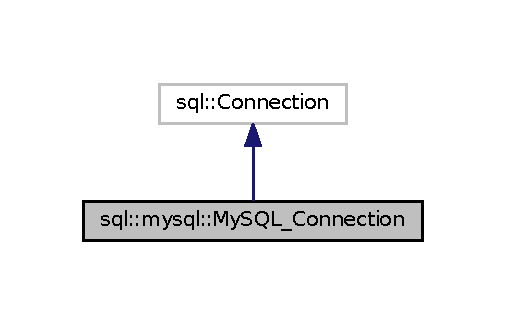
\includegraphics[width=243pt]{classsql_1_1mysql_1_1MySQL__Connection__inherit__graph}
\end{center}
\end{figure}


Graphe de collaboration de sql\+:\+:mysql\+:\+:My\+S\+Q\+L\+\_\+\+Connection\+:\nopagebreak
\begin{figure}[H]
\begin{center}
\leavevmode
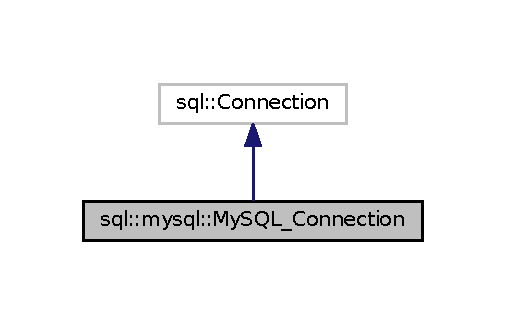
\includegraphics[width=243pt]{classsql_1_1mysql_1_1MySQL__Connection__coll__graph}
\end{center}
\end{figure}
\subsection*{Fonctions membres publiques}
\begin{DoxyCompactItemize}
\item 
{\bfseries My\+S\+Q\+L\+\_\+\+Connection} (Driver $\ast$\+\_\+driver,\+::sql\+::mysql\+::\+Native\+A\+P\+I\+::\+Native\+Connection\+Wrapper \&\+\_\+proxy, const sql\+::\+S\+Q\+L\+String \&host\+Name, const sql\+::\+S\+Q\+L\+String \&user\+Name, const sql\+::\+S\+Q\+L\+String \&password)\hypertarget{classsql_1_1mysql_1_1MySQL__Connection_ac416ee488b73f8d76e3a06388221a129}{}\label{classsql_1_1mysql_1_1MySQL__Connection_ac416ee488b73f8d76e3a06388221a129}

\item 
{\bfseries My\+S\+Q\+L\+\_\+\+Connection} (Driver $\ast$\+\_\+driver,\+::sql\+::mysql\+::\+Native\+A\+P\+I\+::\+Native\+Connection\+Wrapper \&\+\_\+proxy, std\+::map$<$ sql\+::\+S\+Q\+L\+String, sql\+::\+Connect\+Property\+Val $>$ \&options)\hypertarget{classsql_1_1mysql_1_1MySQL__Connection_a4365bfd56d803258f9ed47d95eafaf56}{}\label{classsql_1_1mysql_1_1MySQL__Connection_a4365bfd56d803258f9ed47d95eafaf56}

\item 
void {\bfseries clear\+Warnings} ()\hypertarget{classsql_1_1mysql_1_1MySQL__Connection_aa792ed9b722ec4b45842872865fcc1d9}{}\label{classsql_1_1mysql_1_1MySQL__Connection_aa792ed9b722ec4b45842872865fcc1d9}

\item 
void {\bfseries close} ()\hypertarget{classsql_1_1mysql_1_1MySQL__Connection_aa8d0be382f89bfe031d276a2c67bb7fb}{}\label{classsql_1_1mysql_1_1MySQL__Connection_aa8d0be382f89bfe031d276a2c67bb7fb}

\item 
void {\bfseries commit} ()\hypertarget{classsql_1_1mysql_1_1MySQL__Connection_aca3dab58cd10c2bd877fadc2fa7b9b3f}{}\label{classsql_1_1mysql_1_1MySQL__Connection_aca3dab58cd10c2bd877fadc2fa7b9b3f}

\item 
sql\+::\+Statement $\ast$ {\bfseries create\+Statement} ()\hypertarget{classsql_1_1mysql_1_1MySQL__Connection_a65dd9ce62b91f6ee7422bf6acaa6dc59}{}\label{classsql_1_1mysql_1_1MySQL__Connection_a65dd9ce62b91f6ee7422bf6acaa6dc59}

\item 
sql\+::\+S\+Q\+L\+String {\bfseries escape\+String} (const sql\+::\+S\+Q\+L\+String \&)\hypertarget{classsql_1_1mysql_1_1MySQL__Connection_a4ab19794fc96f0b771dc7f3a9b89d445}{}\label{classsql_1_1mysql_1_1MySQL__Connection_a4ab19794fc96f0b771dc7f3a9b89d445}

\item 
bool {\bfseries get\+Auto\+Commit} ()\hypertarget{classsql_1_1mysql_1_1MySQL__Connection_aa8a7c0dfd9b9dd7f8c00c43fefa2f8a4}{}\label{classsql_1_1mysql_1_1MySQL__Connection_aa8a7c0dfd9b9dd7f8c00c43fefa2f8a4}

\item 
sql\+::\+S\+Q\+L\+String {\bfseries get\+Catalog} ()\hypertarget{classsql_1_1mysql_1_1MySQL__Connection_af410a283060804936031001d38f89e9b}{}\label{classsql_1_1mysql_1_1MySQL__Connection_af410a283060804936031001d38f89e9b}

\item 
Driver $\ast$ {\bfseries get\+Driver} ()\hypertarget{classsql_1_1mysql_1_1MySQL__Connection_af4aaa6f7a2564e6cd7b259a24fe8f0ef}{}\label{classsql_1_1mysql_1_1MySQL__Connection_af4aaa6f7a2564e6cd7b259a24fe8f0ef}

\item 
sql\+::\+S\+Q\+L\+String {\bfseries get\+Schema} ()\hypertarget{classsql_1_1mysql_1_1MySQL__Connection_a49bf51d2c4586f8f85c362a6c71cf8b6}{}\label{classsql_1_1mysql_1_1MySQL__Connection_a49bf51d2c4586f8f85c362a6c71cf8b6}

\item 
sql\+::\+S\+Q\+L\+String {\bfseries get\+Client\+Info} ()\hypertarget{classsql_1_1mysql_1_1MySQL__Connection_aa94814c22d27fae1f62f8a077619026c}{}\label{classsql_1_1mysql_1_1MySQL__Connection_aa94814c22d27fae1f62f8a077619026c}

\item 
void {\bfseries get\+Client\+Option} (const sql\+::\+S\+Q\+L\+String \&option\+Name, void $\ast$option\+Value)\hypertarget{classsql_1_1mysql_1_1MySQL__Connection_a0c80ccabb9723fc4e7bcbe1fac2b7cbf}{}\label{classsql_1_1mysql_1_1MySQL__Connection_a0c80ccabb9723fc4e7bcbe1fac2b7cbf}

\item 
sql\+::\+S\+Q\+L\+String {\bfseries get\+Client\+Option} (const sql\+::\+S\+Q\+L\+String \&option\+Name)\hypertarget{classsql_1_1mysql_1_1MySQL__Connection_a6aa6995181dd5acfa0c18ec7917d2d02}{}\label{classsql_1_1mysql_1_1MySQL__Connection_a6aa6995181dd5acfa0c18ec7917d2d02}

\item 
sql\+::\+Database\+Meta\+Data $\ast$ {\bfseries get\+Meta\+Data} ()\hypertarget{classsql_1_1mysql_1_1MySQL__Connection_a5fcfd3fa9932acb64c36d49c0e264e95}{}\label{classsql_1_1mysql_1_1MySQL__Connection_a5fcfd3fa9932acb64c36d49c0e264e95}

\item 
enum\+\_\+transaction\+\_\+isolation {\bfseries get\+Transaction\+Isolation} ()\hypertarget{classsql_1_1mysql_1_1MySQL__Connection_a556dcab3c0deb14fde548a270d9168ad}{}\label{classsql_1_1mysql_1_1MySQL__Connection_a556dcab3c0deb14fde548a270d9168ad}

\item 
const S\+Q\+L\+Warning $\ast$ {\bfseries get\+Warnings} ()\hypertarget{classsql_1_1mysql_1_1MySQL__Connection_a62b556bf59e83dae5bafd52cce4801a7}{}\label{classsql_1_1mysql_1_1MySQL__Connection_a62b556bf59e83dae5bafd52cce4801a7}

\item 
bool {\bfseries is\+Closed} ()\hypertarget{classsql_1_1mysql_1_1MySQL__Connection_a00820cf65fea6a9fd9cb936a6781db33}{}\label{classsql_1_1mysql_1_1MySQL__Connection_a00820cf65fea6a9fd9cb936a6781db33}

\item 
bool {\bfseries is\+Read\+Only} ()\hypertarget{classsql_1_1mysql_1_1MySQL__Connection_af395e4c12315d0dcf9e3a5abbcbb33e2}{}\label{classsql_1_1mysql_1_1MySQL__Connection_af395e4c12315d0dcf9e3a5abbcbb33e2}

\item 
bool {\bfseries is\+Valid} ()\hypertarget{classsql_1_1mysql_1_1MySQL__Connection_a081337e746b0eabcf0a7cb136b50277b}{}\label{classsql_1_1mysql_1_1MySQL__Connection_a081337e746b0eabcf0a7cb136b50277b}

\item 
bool {\bfseries reconnect} ()\hypertarget{classsql_1_1mysql_1_1MySQL__Connection_a19ebafbbc4bc37958bcc93c7fa0807e9}{}\label{classsql_1_1mysql_1_1MySQL__Connection_a19ebafbbc4bc37958bcc93c7fa0807e9}

\item 
sql\+::\+S\+Q\+L\+String {\bfseries native\+S\+QL} (const sql\+::\+S\+Q\+L\+String \&sql)\hypertarget{classsql_1_1mysql_1_1MySQL__Connection_a7242075ae362ec3fbe65194f7043abc4}{}\label{classsql_1_1mysql_1_1MySQL__Connection_a7242075ae362ec3fbe65194f7043abc4}

\item 
sql\+::\+Prepared\+Statement $\ast$ {\bfseries prepare\+Statement} (const sql\+::\+S\+Q\+L\+String \&sql)\hypertarget{classsql_1_1mysql_1_1MySQL__Connection_a5d4ab19b238692240183b849c84c2166}{}\label{classsql_1_1mysql_1_1MySQL__Connection_a5d4ab19b238692240183b849c84c2166}

\item 
sql\+::\+Prepared\+Statement $\ast$ {\bfseries prepare\+Statement} (const sql\+::\+S\+Q\+L\+String \&sql, int auto\+Generated\+Keys)\hypertarget{classsql_1_1mysql_1_1MySQL__Connection_a4b341cf31b1fadb55fa573d5fc570de7}{}\label{classsql_1_1mysql_1_1MySQL__Connection_a4b341cf31b1fadb55fa573d5fc570de7}

\item 
sql\+::\+Prepared\+Statement $\ast$ {\bfseries prepare\+Statement} (const sql\+::\+S\+Q\+L\+String \&sql, int column\+Indexes\mbox{[}$\,$\mbox{]})\hypertarget{classsql_1_1mysql_1_1MySQL__Connection_a02a26ce23b897f09189ddafd4b87849e}{}\label{classsql_1_1mysql_1_1MySQL__Connection_a02a26ce23b897f09189ddafd4b87849e}

\item 
sql\+::\+Prepared\+Statement $\ast$ {\bfseries prepare\+Statement} (const sql\+::\+S\+Q\+L\+String \&sql, int result\+Set\+Type, int result\+Set\+Concurrency)\hypertarget{classsql_1_1mysql_1_1MySQL__Connection_afcddea07aca0542a2a6e814ba1ee4bd6}{}\label{classsql_1_1mysql_1_1MySQL__Connection_afcddea07aca0542a2a6e814ba1ee4bd6}

\item 
sql\+::\+Prepared\+Statement $\ast$ {\bfseries prepare\+Statement} (const sql\+::\+S\+Q\+L\+String \&sql, int result\+Set\+Type, int result\+Set\+Concurrency, int result\+Set\+Holdability)\hypertarget{classsql_1_1mysql_1_1MySQL__Connection_a156ab360753b8b1ca11682422d9914b3}{}\label{classsql_1_1mysql_1_1MySQL__Connection_a156ab360753b8b1ca11682422d9914b3}

\item 
sql\+::\+Prepared\+Statement $\ast$ {\bfseries prepare\+Statement} (const sql\+::\+S\+Q\+L\+String \&sql, sql\+::\+S\+Q\+L\+String column\+Names\mbox{[}$\,$\mbox{]})\hypertarget{classsql_1_1mysql_1_1MySQL__Connection_a27a07ce9777574a0592fe6f8834e082f}{}\label{classsql_1_1mysql_1_1MySQL__Connection_a27a07ce9777574a0592fe6f8834e082f}

\item 
void {\bfseries release\+Savepoint} (Savepoint $\ast$savepoint)\hypertarget{classsql_1_1mysql_1_1MySQL__Connection_af85e740e1d7cc9f16d357afdd9f4419d}{}\label{classsql_1_1mysql_1_1MySQL__Connection_af85e740e1d7cc9f16d357afdd9f4419d}

\item 
void {\bfseries rollback} ()\hypertarget{classsql_1_1mysql_1_1MySQL__Connection_a30102a74e65a62cff9c36ce77a8c7f44}{}\label{classsql_1_1mysql_1_1MySQL__Connection_a30102a74e65a62cff9c36ce77a8c7f44}

\item 
void {\bfseries rollback} (Savepoint $\ast$savepoint)\hypertarget{classsql_1_1mysql_1_1MySQL__Connection_a64fc3a6f403a19fee712142141a07ef4}{}\label{classsql_1_1mysql_1_1MySQL__Connection_a64fc3a6f403a19fee712142141a07ef4}

\item 
void {\bfseries set\+Auto\+Commit} (bool auto\+Commit)\hypertarget{classsql_1_1mysql_1_1MySQL__Connection_a66dd8515ee9ccfe186fc1d2b597f220f}{}\label{classsql_1_1mysql_1_1MySQL__Connection_a66dd8515ee9ccfe186fc1d2b597f220f}

\item 
void {\bfseries set\+Catalog} (const sql\+::\+S\+Q\+L\+String \&catalog)\hypertarget{classsql_1_1mysql_1_1MySQL__Connection_a85487982563f163064269bbe072bf2a0}{}\label{classsql_1_1mysql_1_1MySQL__Connection_a85487982563f163064269bbe072bf2a0}

\item 
void {\bfseries set\+Schema} (const sql\+::\+S\+Q\+L\+String \&catalog)\hypertarget{classsql_1_1mysql_1_1MySQL__Connection_ae9c04f366688e047e898487bc6fd6e1b}{}\label{classsql_1_1mysql_1_1MySQL__Connection_ae9c04f366688e047e898487bc6fd6e1b}

\item 
sql\+::\+Connection $\ast$ {\bfseries set\+Client\+Option} (const sql\+::\+S\+Q\+L\+String \&option\+Name, const void $\ast$option\+Value)\hypertarget{classsql_1_1mysql_1_1MySQL__Connection_a146973ddeaf89e344b719cefb09c55ad}{}\label{classsql_1_1mysql_1_1MySQL__Connection_a146973ddeaf89e344b719cefb09c55ad}

\item 
sql\+::\+Connection $\ast$ {\bfseries set\+Client\+Option} (const sql\+::\+S\+Q\+L\+String \&option\+Name, const sql\+::\+S\+Q\+L\+String \&option\+Value)\hypertarget{classsql_1_1mysql_1_1MySQL__Connection_a2e01fff22d660d797501ac29e9a436e7}{}\label{classsql_1_1mysql_1_1MySQL__Connection_a2e01fff22d660d797501ac29e9a436e7}

\item 
void {\bfseries set\+Holdability} (int holdability)\hypertarget{classsql_1_1mysql_1_1MySQL__Connection_a4703a47ce23ba73ec2fadfc680b2e868}{}\label{classsql_1_1mysql_1_1MySQL__Connection_a4703a47ce23ba73ec2fadfc680b2e868}

\item 
void {\bfseries set\+Read\+Only} (bool read\+Only)\hypertarget{classsql_1_1mysql_1_1MySQL__Connection_ac4bafbedfb801fa73694ddbfca4a95c6}{}\label{classsql_1_1mysql_1_1MySQL__Connection_ac4bafbedfb801fa73694ddbfca4a95c6}

\item 
sql\+::\+Savepoint $\ast$ {\bfseries set\+Savepoint} ()\hypertarget{classsql_1_1mysql_1_1MySQL__Connection_afca8998459c9f06788b3ed3be25b81de}{}\label{classsql_1_1mysql_1_1MySQL__Connection_afca8998459c9f06788b3ed3be25b81de}

\item 
sql\+::\+Savepoint $\ast$ {\bfseries set\+Savepoint} (const sql\+::\+S\+Q\+L\+String \&name)\hypertarget{classsql_1_1mysql_1_1MySQL__Connection_a2d0045db252b83fd0222e716f9bfc71d}{}\label{classsql_1_1mysql_1_1MySQL__Connection_a2d0045db252b83fd0222e716f9bfc71d}

\item 
void {\bfseries set\+Transaction\+Isolation} (enum\+\_\+transaction\+\_\+isolation level)\hypertarget{classsql_1_1mysql_1_1MySQL__Connection_a50c5f85205c2333804ee503778ed05b0}{}\label{classsql_1_1mysql_1_1MySQL__Connection_a50c5f85205c2333804ee503778ed05b0}

\item 
virtual sql\+::\+S\+Q\+L\+String {\bfseries get\+Session\+Variable} (const sql\+::\+S\+Q\+L\+String \&varname)\hypertarget{classsql_1_1mysql_1_1MySQL__Connection_ae35fdfcee5de39dc2ec759bc5b8145be}{}\label{classsql_1_1mysql_1_1MySQL__Connection_ae35fdfcee5de39dc2ec759bc5b8145be}

\item 
virtual void {\bfseries set\+Session\+Variable} (const sql\+::\+S\+Q\+L\+String \&varname, const sql\+::\+S\+Q\+L\+String \&value)\hypertarget{classsql_1_1mysql_1_1MySQL__Connection_a5e3eb3eed3d7092c9d03efd7d52629c2}{}\label{classsql_1_1mysql_1_1MySQL__Connection_a5e3eb3eed3d7092c9d03efd7d52629c2}

\item 
virtual void {\bfseries set\+Session\+Variable} (const sql\+::\+S\+Q\+L\+String \&varname, unsigned int value)\hypertarget{classsql_1_1mysql_1_1MySQL__Connection_ad8a42ed4da0fb3810a7624cc969d7ced}{}\label{classsql_1_1mysql_1_1MySQL__Connection_ad8a42ed4da0fb3810a7624cc969d7ced}

\item 
virtual sql\+::\+S\+Q\+L\+String {\bfseries get\+Last\+Statement\+Info} ()\hypertarget{classsql_1_1mysql_1_1MySQL__Connection_a31744f8fd6beaa9c488f947962c1bae6}{}\label{classsql_1_1mysql_1_1MySQL__Connection_a31744f8fd6beaa9c488f947962c1bae6}

\end{DoxyCompactItemize}


La documentation de cette classe a été générée à partir du fichier suivant \+:\begin{DoxyCompactItemize}
\item 
mysql\+\_\+connection.\+h\end{DoxyCompactItemize}

\hypertarget{classsql_1_1mysql_1_1MySQL__Savepoint}{}\section{Référence de la classe sql\+:\+:mysql\+:\+:My\+S\+Q\+L\+\_\+\+Savepoint}
\label{classsql_1_1mysql_1_1MySQL__Savepoint}\index{sql\+::mysql\+::\+My\+S\+Q\+L\+\_\+\+Savepoint@{sql\+::mysql\+::\+My\+S\+Q\+L\+\_\+\+Savepoint}}


Graphe d\textquotesingle{}héritage de sql\+:\+:mysql\+:\+:My\+S\+Q\+L\+\_\+\+Savepoint\+:\nopagebreak
\begin{figure}[H]
\begin{center}
\leavevmode
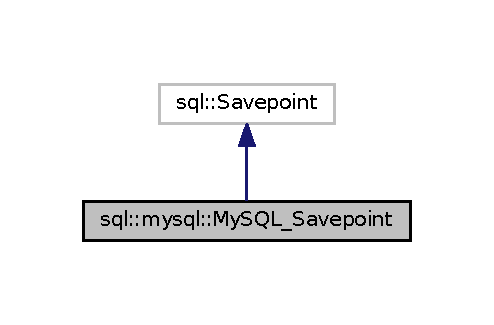
\includegraphics[width=237pt]{classsql_1_1mysql_1_1MySQL__Savepoint__inherit__graph}
\end{center}
\end{figure}


Graphe de collaboration de sql\+:\+:mysql\+:\+:My\+S\+Q\+L\+\_\+\+Savepoint\+:\nopagebreak
\begin{figure}[H]
\begin{center}
\leavevmode
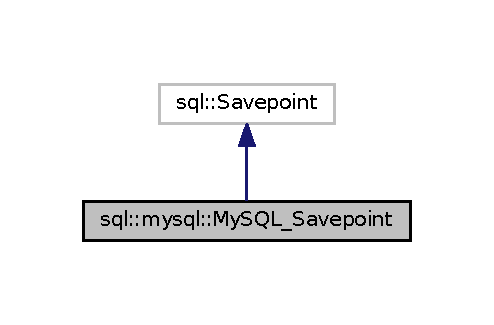
\includegraphics[width=237pt]{classsql_1_1mysql_1_1MySQL__Savepoint__coll__graph}
\end{center}
\end{figure}
\subsection*{Fonctions membres publiques}
\begin{DoxyCompactItemize}
\item 
{\bfseries My\+S\+Q\+L\+\_\+\+Savepoint} (const sql\+::\+S\+Q\+L\+String \&savepoint)\hypertarget{classsql_1_1mysql_1_1MySQL__Savepoint_a864a5455837699c737623060010dd7b5}{}\label{classsql_1_1mysql_1_1MySQL__Savepoint_a864a5455837699c737623060010dd7b5}

\item 
int {\bfseries get\+Savepoint\+Id} ()\hypertarget{classsql_1_1mysql_1_1MySQL__Savepoint_a0fb4031dfa691e3f2453c2d9eff5ea09}{}\label{classsql_1_1mysql_1_1MySQL__Savepoint_a0fb4031dfa691e3f2453c2d9eff5ea09}

\item 
sql\+::\+S\+Q\+L\+String {\bfseries get\+Savepoint\+Name} ()\hypertarget{classsql_1_1mysql_1_1MySQL__Savepoint_a7c2aeca2f1c37da2ae0fe213eb9e6b40}{}\label{classsql_1_1mysql_1_1MySQL__Savepoint_a7c2aeca2f1c37da2ae0fe213eb9e6b40}

\end{DoxyCompactItemize}


La documentation de cette classe a été générée à partir du fichier suivant \+:\begin{DoxyCompactItemize}
\item 
mysql\+\_\+connection.\+h\end{DoxyCompactItemize}

\hypertarget{structqt__meta__stringdata__EchoClient__t}{}\section{Référence de la structure qt\+\_\+meta\+\_\+stringdata\+\_\+\+Echo\+Client\+\_\+t}
\label{structqt__meta__stringdata__EchoClient__t}\index{qt\+\_\+meta\+\_\+stringdata\+\_\+\+Echo\+Client\+\_\+t@{qt\+\_\+meta\+\_\+stringdata\+\_\+\+Echo\+Client\+\_\+t}}
\subsection*{Attributs publics}
\begin{DoxyCompactItemize}
\item 
Q\+Byte\+Array\+Data {\bfseries data} \mbox{[}6\mbox{]}\hypertarget{structqt__meta__stringdata__EchoClient__t_a7b2bbb612d8683c72c829480006e0640}{}\label{structqt__meta__stringdata__EchoClient__t_a7b2bbb612d8683c72c829480006e0640}

\item 
char {\bfseries stringdata0} \mbox{[}61\mbox{]}\hypertarget{structqt__meta__stringdata__EchoClient__t_a16c89302790e0ee63ddb4dd7fbae4f57}{}\label{structqt__meta__stringdata__EchoClient__t_a16c89302790e0ee63ddb4dd7fbae4f57}

\end{DoxyCompactItemize}


La documentation de cette structure a été générée à partir du fichier suivant \+:\begin{DoxyCompactItemize}
\item 
moc\+\_\+echoclient.\+cpp\end{DoxyCompactItemize}

\chapter{Documentation des fichiers}
\hypertarget{database_8cpp}{}\section{Référence du fichier database.\+cpp}
\label{database_8cpp}\index{database.\+cpp@{database.\+cpp}}
{\ttfamily \#include \char`\"{}database.\+h\char`\"{}}\\*
Graphe des dépendances par inclusion de database.\+cpp\+:
\nopagebreak
\begin{figure}[H]
\begin{center}
\leavevmode
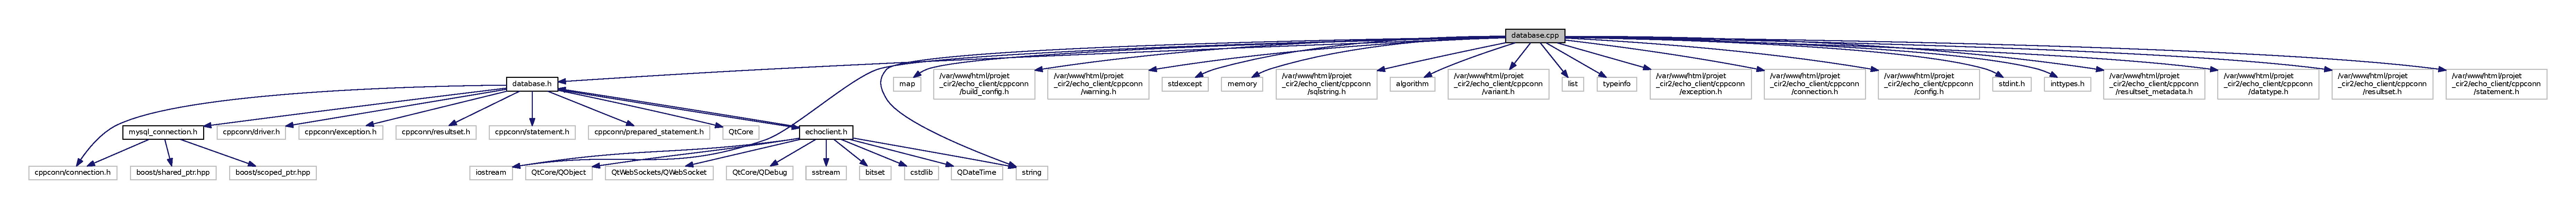
\includegraphics[width=350pt]{database_8cpp__incl}
\end{center}
\end{figure}

\hypertarget{echoclient_8cpp}{}\section{Référence du fichier echoclient.\+cpp}
\label{echoclient_8cpp}\index{echoclient.\+cpp@{echoclient.\+cpp}}
{\ttfamily \#include \char`\"{}echoclient.\+h\char`\"{}}\\*
{\ttfamily \#include \char`\"{}database.\+h\char`\"{}}\\*
{\ttfamily \#include $<$sstream$>$}\\*
{\ttfamily \#include $<$Q\+Json\+Document$>$}\\*
{\ttfamily \#include $<$Q\+Json\+Object$>$}\\*
{\ttfamily \#include $<$Q\+Json\+Value$>$}\\*
{\ttfamily \#include $<$Q\+Json\+Array$>$}\\*
{\ttfamily \#include $<$string$>$}\\*
{\ttfamily \#include $<$iostream$>$}\\*
Graphe des dépendances par inclusion de echoclient.\+cpp\+:\nopagebreak
\begin{figure}[H]
\begin{center}
\leavevmode
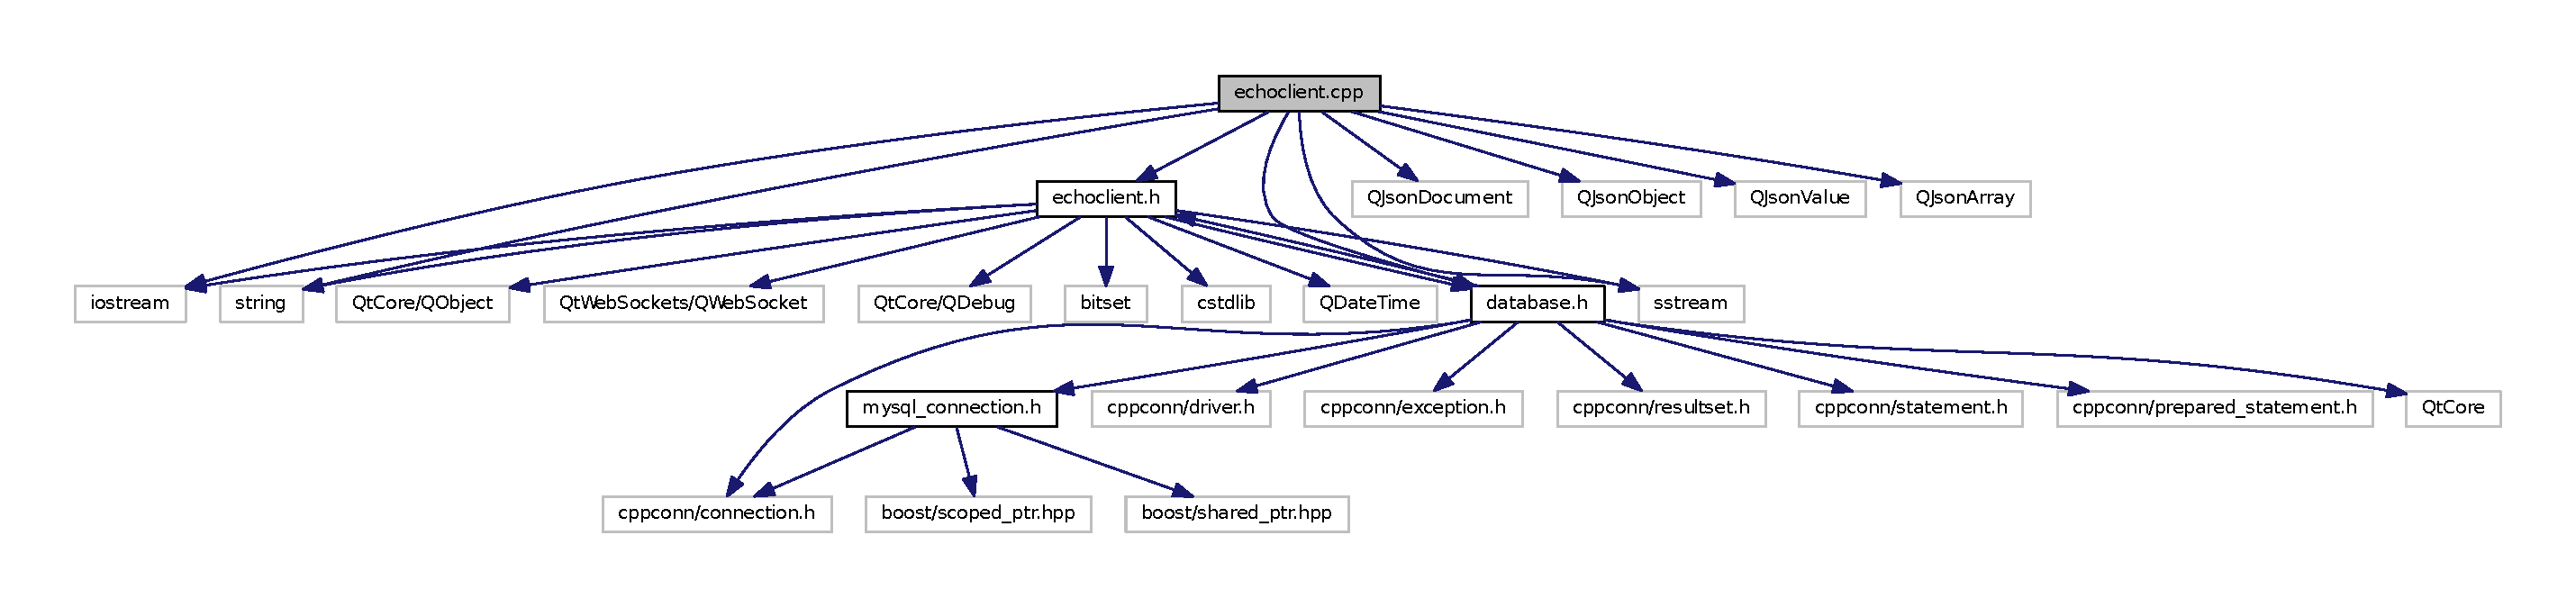
\includegraphics[width=350pt]{echoclient_8cpp__incl}
\end{center}
\end{figure}

\hypertarget{echoclient_8h}{}\section{Référence du fichier echoclient.\+h}
\label{echoclient_8h}\index{echoclient.\+h@{echoclient.\+h}}


Le fichier d\textquotesingle{}en-\/tête de la classe {\bfseries \hyperlink{classDataBase}{Data\+Base}}.  


{\ttfamily \#include $<$Qt\+Core/\+Q\+Object$>$}\\*
{\ttfamily \#include $<$Qt\+Web\+Sockets/\+Q\+Web\+Socket$>$}\\*
{\ttfamily \#include $<$iostream$>$}\\*
{\ttfamily \#include $<$Qt\+Core/\+Q\+Debug$>$}\\*
{\ttfamily \#include $<$string$>$}\\*
{\ttfamily \#include $<$sstream$>$}\\*
{\ttfamily \#include $<$bitset$>$}\\*
{\ttfamily \#include $<$cstdlib$>$}\\*
{\ttfamily \#include $<$Q\+Date\+Time$>$}\\*
{\ttfamily \#include \char`\"{}database.\+h\char`\"{}}\\*
Graphe des dépendances par inclusion de echoclient.\+h\+:\nopagebreak
\begin{figure}[H]
\begin{center}
\leavevmode
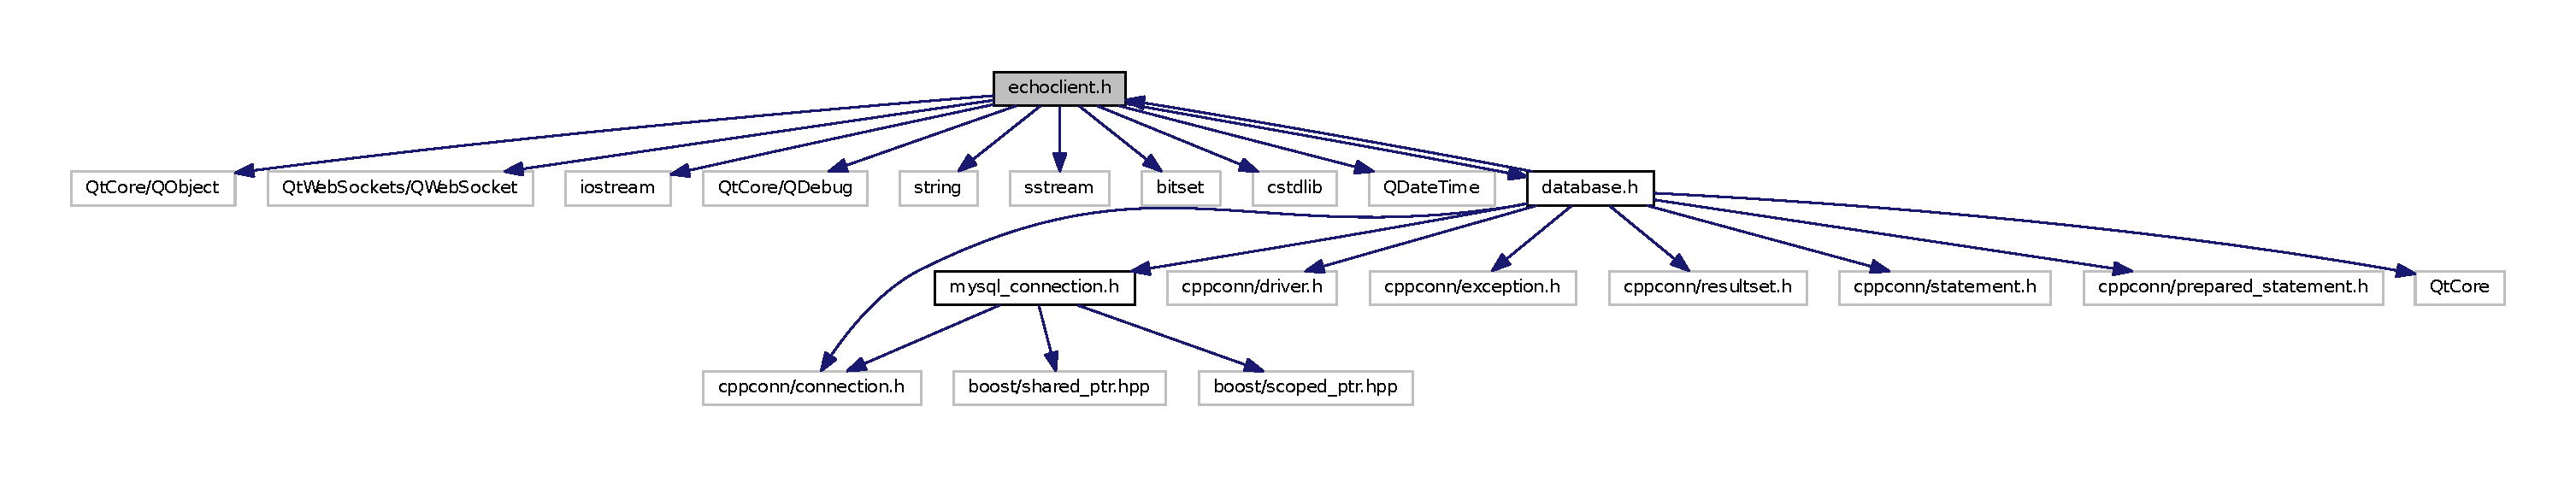
\includegraphics[width=350pt]{echoclient_8h__incl}
\end{center}
\end{figure}
Ce graphe montre quels fichiers incluent directement ou indirectement ce fichier \+:
\nopagebreak
\begin{figure}[H]
\begin{center}
\leavevmode
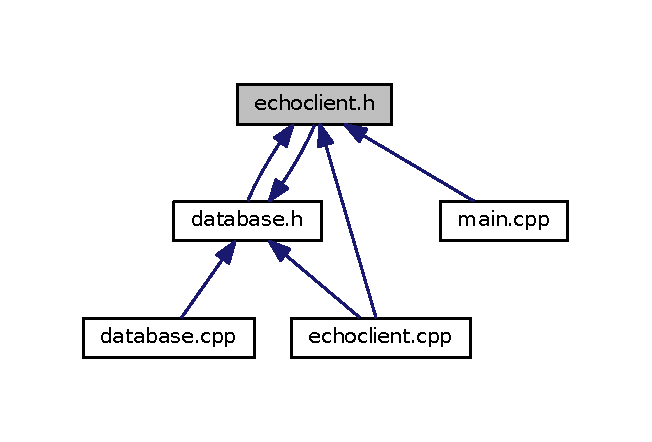
\includegraphics[width=313pt]{echoclient_8h__dep__incl}
\end{center}
\end{figure}
\subsection*{Classes}
\begin{DoxyCompactItemize}
\item 
class \hyperlink{classEchoClient}{Echo\+Client}
\begin{DoxyCompactList}\small\item\em La classe {\bfseries \hyperlink{classEchoClient}{Echo\+Client}} est l\textquotesingle{}ensemble des fonctionnalités permettant de récupérer une trame et de la traiter. \end{DoxyCompactList}\end{DoxyCompactItemize}


\subsection{Description détaillée}
Le fichier d\textquotesingle{}en-\/tête de la classe {\bfseries \hyperlink{classDataBase}{Data\+Base}}. 

Le fichier d\textquotesingle{}en-\/tête correspondant à la classe {\bfseries \hyperlink{classEchoClient}{Echo\+Client}}.

\begin{DoxyAuthor}{Auteur}
Steve Corre et Benjamin Binard 
\end{DoxyAuthor}

\hypertarget{main_8cpp}{}\section{Référence du fichier main.\+cpp}
\label{main_8cpp}\index{main.\+cpp@{main.\+cpp}}
{\ttfamily \#include $<$Qt\+Core/\+Q\+Core\+Application$>$}\\*
{\ttfamily \#include $<$Qt\+Core/\+Q\+Command\+Line\+Parser$>$}\\*
{\ttfamily \#include $<$Qt\+Core/\+Q\+Command\+Line\+Option$>$}\\*
{\ttfamily \#include \char`\"{}echoclient.\+h\char`\"{}}\\*
Graphe des dépendances par inclusion de main.\+cpp\+:
\nopagebreak
\begin{figure}[H]
\begin{center}
\leavevmode
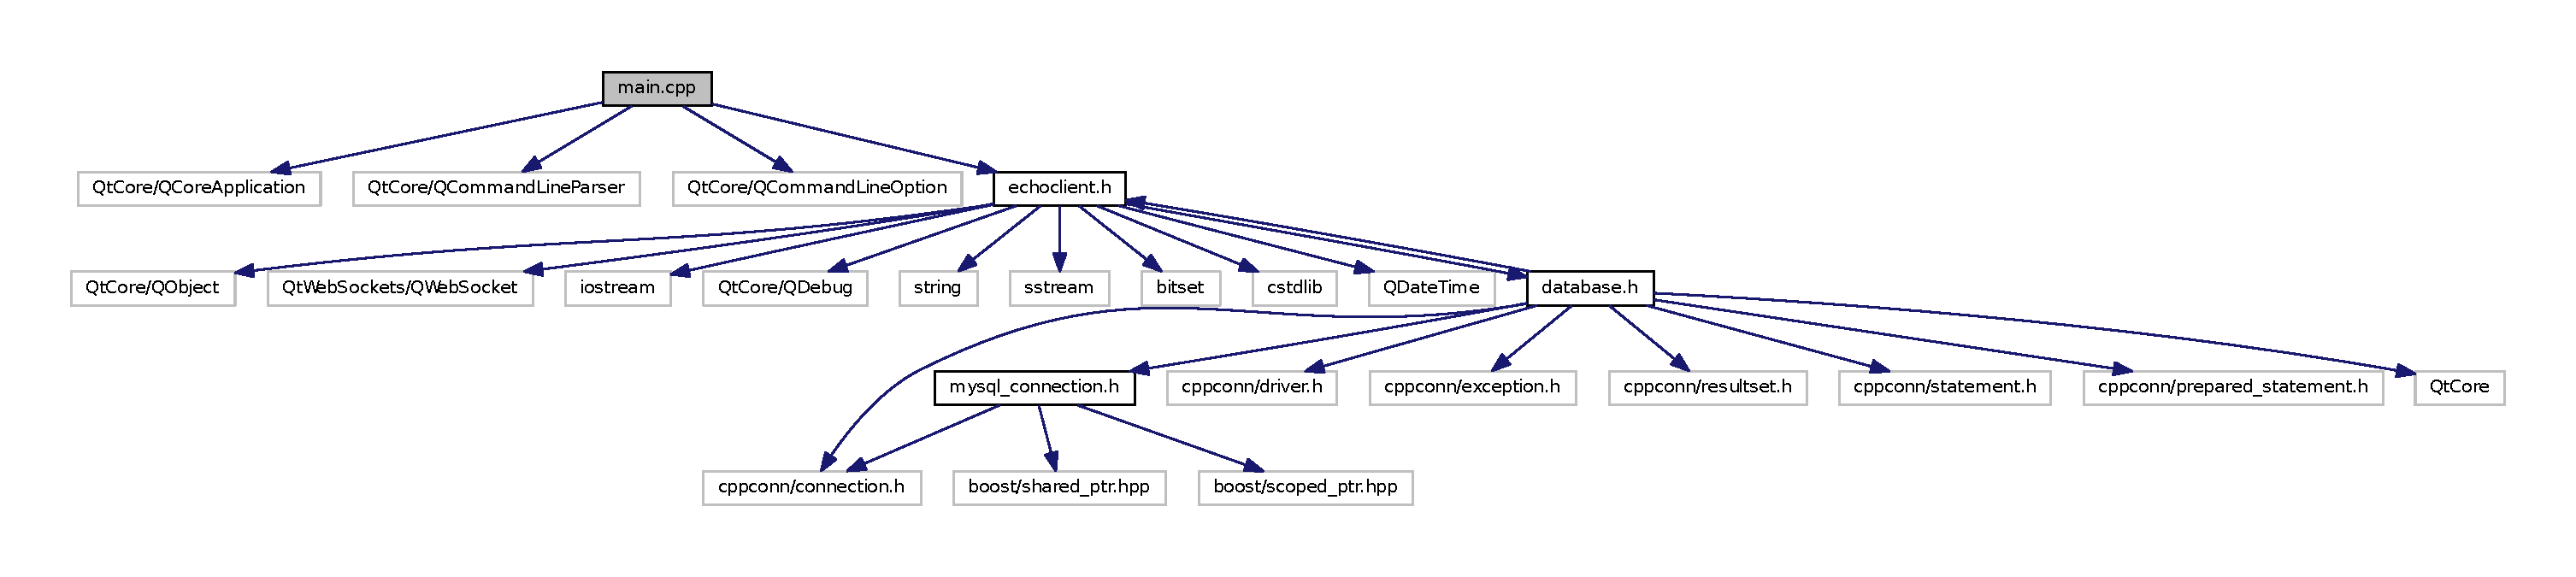
\includegraphics[width=350pt]{main_8cpp__incl}
\end{center}
\end{figure}
\subsection*{Fonctions}
\begin{DoxyCompactItemize}
\item 
int {\bfseries main} (int argc, char $\ast$argv\mbox{[}$\,$\mbox{]})\hypertarget{main_8cpp_a0ddf1224851353fc92bfbff6f499fa97}{}\label{main_8cpp_a0ddf1224851353fc92bfbff6f499fa97}

\end{DoxyCompactItemize}

%--- End generated contents ---

% Index
\backmatter
\newpage
\phantomsection
\clearemptydoublepage
\addcontentsline{toc}{chapter}{Index}
\printindex

\end{document}
